\documentclass[mathNotesPreamble]{subfiles}
\begin{document}
%\relscale{1.4} %TODO
\section{13.2: Vectors in Three Dimensions}~

  \textbf{The $xyz$- Coordinate System:}\newline
    The three-dimensional coordinate system is created by adding the $z$-axis, which is perpendicular to both the $x$-axis and the $y$-axis. When looking at the $xy$-plane, the positive direction of the $z$-axis protrudes towards the viewer. This can also be shown using the right-hand rule (Figure 13.25 from Briggs):
    \begin{center}
      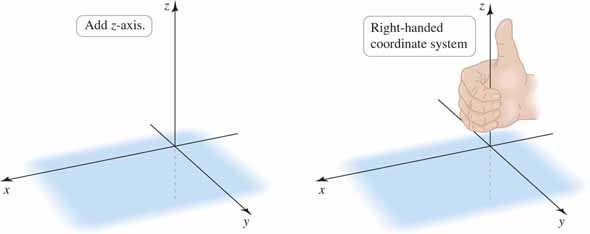
\includegraphics[width=0.7\linewidth]{images/briggs_13_02/fig13_25}
    \end{center}
    \vspace*{\stretch{1}}

    \begin{defn*}
      \begin{minipage}{0.5\linewidth}
        This three-dimensional coordinate system is broken up into eight \textbf{octants}, which are separated by
        \begin{itemize}
          \item the \textbf{$xy$-plane} ($z=0$),
          \item the \textbf{$xz$-plane} ($y=0$), and
          \item the \textbf{$yz$-plane} ($x=0$).
        \end{itemize}
           The \textbf{origin} is the location where all three axes intersect.
      \end{minipage}%
      \begin{minipage}{0.5\linewidth}
        \vspace*{-\baselineskip}
        \begin{flushright}
          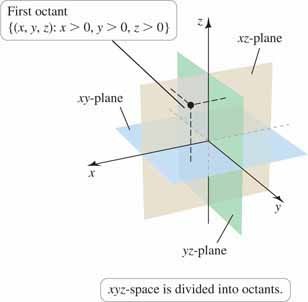
\includegraphics[width=0.85\linewidth]{images/briggs_13_02/fig13_26}
        \end{flushright}
      \end{minipage}%
    \end{defn*}
    \vspace*{\stretch{1}}
    \pagebreak
    %TODO insert examples of plotting points in 3D

  \textbf{Equations of Simple Planes:}\newline
    Planes in three-dimensions are analogous to lines in two-dimensions. Below, we see the $yz$-plane, the $xz$-plane, and the $xy$-plane, along with planes that are parallel where $x$, $y$, and $z$ are fixed respectively:
    \begin{center}
      \begin{tikzpicture}[scale=0.8, declare function={
        xyPlane(\x,\y,\z)=;
        xzPlane(\x,\y,\z)=;
        yzPlane(\x,\y,\z)=;
        }]
        \begin{groupplot}[
          group style={group size=3 by 1, horizontal sep=1cm},
          axis lines=center,
          axis line style={black,->},
          xmin=0, xmax=5.5, xticklabels={,,,},
          ymin=0, ymax=5.5, yticklabels={,,,},
          zmin=0, zmax=5.5, zticklabels={,,,},
          ticklabel style={font=\normalsize,inner sep=0.5pt,fill=white,opacity=0.75, text opacity=1},
          xlabel=$x$, xlabel style={at={(ticklabel* cs:1)},anchor=north east},
          ylabel=$y$, ylabel style={at={(ticklabel* cs:1)},anchor=west},
          zlabel=$z$, zlabel style={at={(ticklabel* cs:1)},anchor=south},
          view={120}{27.5},
          ]
          \nextgroupplot
            \addplot3[soldot, black] coordinates{(3,0,0)} 
              node[below, xshift=10pt, yshift=-5pt, font=\Large] {$(3,0,0)$};
            \addplot3[no marks,draw=none, fill=ClemsonPurple!60, opacity=0.5] 
              coordinates {(0,0,0) (0,0,4) (0,4,4) (0,4,0)} 
              node[text opacity=1] at (0,2,4.675) {$x=0$};
           \addplot3[no marks,draw=none, fill=ClemsonPurple, opacity=0.5] 
             coordinates {(3,0,0) (3,0,4) (3,4,4) (3,4,0)} 
             node[text opacity=1] at (3,2,2.25) {$x=3$};
          \nextgroupplot
            \addplot3[soldot, black] coordinates{(0,3,0)} 
              node[above right, font=\Large] {$(0,3,0)$};
            \addplot3[no marks,draw=none, fill=ClemsonOrange!65, opacity=0.5] 
              coordinates {(0,0,0) (0,0,4) (4,0,4) (4,0,0)} 
              node[text opacity=1] at (2,0,2) {$y=0$};
            \addplot3[no marks,draw=none, fill=ClemsonOrange!90, opacity=0.5] 
              coordinates {(0,3,0) (0,3,4) (4,3,4) (4,3,0)}
              node[text opacity=1] at (2,3,2) {$y=3$};
          \nextgroupplot
            \addplot3[soldot, black] coordinates{(0,0,3)} 
              node[above right, font=\Large] {$(0,0,3)$};
            \addplot3[no marks,draw=none, fill=BowmanField!60, opacity=0.5] 
              coordinates {(0,0,0) (4,0,0) (4,4,0) (0,4,0)} 
              node[text opacity=1] at (2,2,0) {$z=0$};
            \addplot3[no marks,draw=none, fill=BowmanField!90, opacity=0.5] 
              coordinates {(0,0,3) (4,0,3) (4,4,3) (0,4,3)} 
              node[text opacity=1] at (2,2,3) {$z=3$};
        \end{groupplot}
      \end{tikzpicture}
    \end{center}
    \vspace*{2\baselineskip}

    \begin{ex*}[Parallel planes]
      Determine the equation of the plane parallel to the $xz$-plane passing through the point $(2,-3,7)$.
    \end{ex*}
    \begin{center}
      \begin{tikzpicture}
        \begin{axis}[
          axis lines=center,
          axis line style={black,<->},
          xmin=-1, xmax=4, xmajorticks=false,
          ymin=-4, ymax=0.5, ymajorticks=false,
          zmin=-1, zmax=8, zmajorticks=false,
          enlargelimits={abs=0.75},
          ticklabel style={font=\normalsize,inner sep=0.5pt,fill=white,opacity=1.0, text opacity=1},
          xlabel=$x$, xlabel style={at={(ticklabel* cs:1)},anchor=north west},
          ylabel=$y$, ylabel style={at={(ticklabel* cs:1)},anchor=south west},
          zlabel=$z$, zlabel style={at={(ticklabel* cs:1)},anchor=south west},
          every axis plot/.append style={line width=0.95pt, color=blue, samples=100},
          view={120}{27.5},
          ]
          \addplot3[dashed,blue] coordinates{(0,0,0) (2,0,0) (2,-3,0) (2,-3,7)};
          \addplot3[dashed,black!50] coordinates{(0,0,0) (2,-3,0)};
          \addplot3[draw=none, fill=ClemsonPurple!50, opacity=0.35]
            coordinates{(0,0,0) (2,0,0) (2,-3,0)};
          \addplot3[dashed,black!50] coordinates{(0,0,0) (2,-3,7)};
          \addplot3[draw=none, fill=ClemsonOrange!50, opacity=0.25]
            coordinates{(0,0,0) (2,-3,0) (2,-3,7)};
          \addplot3[soldot] coordinates{(2,-3,7)}
            node[black, above, font=\normalsize] {$(2,-3,7)$};
        \end{axis}
      \end{tikzpicture}
    \end{center}
    %TODO LC for correct equation
    \vspace*{\stretch{1}}
    \pagebreak

  \textbf{Distances in $xyz$-Space:}\newline
    Recall that in $\bbr^2$, for some vector $\overrightharp{PR}$, the distance formula is given by
      \[\abs{PR}=\sqrt{\parens{x_2-x_1}^2-\parens{y_2-y_1}^2}\]
    where $(x_1,y_1)$ and $(x_2,y_2)$ represent the points $P$ and $R$ respectively.
    This idea can be further extended into $\bbr^3$ by considering the two sides of the triangle formed by the points $P(x_1,y_1,z_1)$ and $Q(x_2,y_2,z_2)$:
    \vspace*{\stretch{1}}

    \begin{center}
      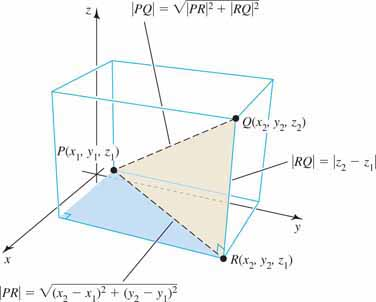
\includegraphics[width=0.5\linewidth]{images/briggs_13_02/fig13_32}
    \end{center}
    \vspace*{\stretch{1}}
    \fbox{\parbox{0.9875\linewidth}{
      \textbf{Distance Formula in $xyz$-Space}

      The \textbf{distance} between points $P(x_1,y_1,z_1)$ and $Q(x_2,y_2,z_2)$ is
        \[\sqrt{\parens{x_2-x_1}^2+\parens{y_2-y_1}^2+\parens{z_2-z_1}^2}\]
      The \textbf{midpoint} between points $P(x_1,y_1,z_1)$ and $Q(x_2,y_2,z_2)$ is found by averaging the $x$-, $y$-, and $z$-coordinates:
        \[\textnormal{Midpoint }=\parens{\frac{x_1+x_2}{2},\frac{y_1+y_2}{2},\frac{z_1+z_2}{2}}\]
    }}
    \pagebreak
    
  \textbf{Equation of a Sphere:}
    \begin{defn*}
      A \textbf{sphere} centered at $(a,b,c)$ with radius $r$ is the set of points satisfying the equation
        \[\parens{x-a}^2+\parens{y-b}^2+\parens{z-c}^2=r^2.\]
      A \textbf{ball} centered at $(a,b,c)$ with radius $r$ is the set of points satisfying the inequality
        \[\parens{x-a}^2+\parens{y-b}^2+\parens{z-c}^2\leq r^2.\]
    \end{defn*}
    
    \begin{ex*}
      Rewrite the following equation into the standard form of a sphere:
        \[x^2+y^2+z^2-2x+6y-8z=-1\]
    \end{ex*}
    %TODO LC to pick center and radius of sphere

  \vspace*{\stretch{1}}
  \textbf{Vector Operations in Terms of Components}
    \begin{defn*}[Vector Operations in $\bbr^3$]
      Suppose $c$ is a scalar, $\bfu=\bracket{u_1,u_2,u_3}$, and $\bfv=\bracket{v_1,v_2,v_3}$.
        \begin{alignat*}{2}
          \bfu+\bfv&=\bracket{u_1+v_1,u_2+v_2,u_3+v_3}&\hspace*{25pt}& \textnormal{\textcolor{blue}{ Vector addition}}\\
          \bfu-\bfv&=\bracket{u_1-v_1,u_2-v_2,u_3-v_3}&& \textnormal{\textcolor{blue}{ Vector subtraction}}\\
          c\bfu&=\bracket{cu_1,cu_2,cu_3}&& \textnormal{\textcolor{blue}{ Scalar multiplication}}
        \end{alignat*}
    \end{defn*}
    
    \pagebreak

  \textbf{Magnitude and Unit Vectors:}\newline
  \begin{defn*}
    The \textbf{magnitude} (or \textbf{length}) of the vector $\overrightharp{PQ}=\bracket{x_2-x_1,y_2-y_1,z_2-z_1}$ is the distance from $P(x_1,y_1,z_1)$ to $Q(x_2,y_2,z_2)$:
      \[\abs{\overrightharp{PQ}}=\sqrt{\parens{x_2-x_1}^2+\parens{y_2-y_1}^2+\parens{z_2-z_1}^2}\]
  \end{defn*}
    

  \begin{center}
    \begin{tikzpicture}[scale=1.0]
      \begin{axis}[
        axis lines=center,
        axis line style={black,->},
        xmin=-0.5, xmax=3, xmajorticks=false,
        ymin=-0.5, ymax=3, ymajorticks=false,
        zmin=-0.5, zmax=3, zmajorticks=false,
        ticklabel style={font=\normalsize,inner sep=1pt,fill=white,opacity=1.0, text opacity=1},
        every axis plot/.append style={line width=0.95pt, color=blue, samples=100},
        view={120}{30},
        ]
        
        \addplot3[fill=ClemsonPurple!75, opacity=0.5, draw=none]
          coordinates{(0.175,0.25,0.4) (1.75,2.675, 3) (1.75,2.675, 0.4)}
          node[above, black, pos=0.285, pin={[pin distance=17pt]-75:{}}, 
          xshift=-2.5pt, yshift=20pt, font=\footnotesize, fill=white, 
          opacity=0.75, inner sep=1pt, text opacity=1] 
          {$\abs{\overrightharp{PQ}}=\sqrt{\parens{x_2-x_1}^2+\parens{y_2-y_1}^2+\parens{z_2-z_1}^2}$};
        \addplot3[black, ->] 
          coordinates{(0.175,0.25,0.4) (1.75,2.675, 3)};
        \addplot3[dashed, black!50] 
          coordinates{(0.175,0.25,0) (0.175,0.25,0.4) (1.75,2.675, 0.4)};
        \addplot3[dashed, black!50] 
          coordinates{(1.75,2.675, 0) (1.75,2.675, 3)};
        \addplot3[soldot,black, mark size=0.75pt] 
          coordinates{(0.175,0.25,0) (1.75,2.675, 0)};
        \addplot3[soldot,black, mark size=0.75pt] 
          coordinates{(0.175,0.25,0.4)} 
          node[above left, font=\normalsize, xshift=-10pt, inner sep=1pt,
          pin={[pin distance=10pt, shorten >=-5pt]-3:{}}]
          {$P(x_1,y_1,z_1)$};
        \addplot3[soldot,black, mark size=0.75pt] 
          coordinates{(1.75,2.675,3)} 
          node[right, font=\normalsize] {$Q(x_2,y_2,z_2)$};
      \end{axis}
    \end{tikzpicture}
  \end{center}
    In $\bbr^3$, the \textbf{coordinate unit vectors} are $\bfi=\bracket{1,0,0}$, $\bfj=\bracket{0,1,0}$, and $\bfk=\bracket{0,0,1}$.
    \pagebreak
    % TODO add examples

  \noindent
  \fbox{\parbox{0.9875\linewidth}{
    \textbf{Properties of Vector Operations:}
    
    Suppose $\bfu$, $\bfv$, and $\bm{w}$ are vectors and $a$ and $c$ are scalars. Then the following properties hold (for vectors in any number of dimensions).
    \begin{center}
      \begin{minipage}{0.925\linewidth}
        \TabPositions{0.425\linewidth}
        \begin{enumerate}
          \item 
            $\bfu+\bfv=\bfv+\bfu$ 
            \tab \textcolor{blue}{Commutative property of addition}
          \item 
            $\parens{\bfu+\bfv}+\bm w=\bfu+\parens{\bfv+\bm w}$
            \tab \textcolor{blue}{Associative property of addition}
          \item 
            $\bfv+\bfO=\bfv$
            \tab \textcolor{blue}{Additive identity}
          \item 
            $\bfv+\parens{-\bfv}=\bfO$
            \tab \textcolor{blue}{Additive inverse}
          \item 
            $c\parens{\bfu+\bfv}=c\bfu+c\bfv$
            \tab \textcolor{blue}{Distributive property 1}
          \item 
            $\parens{a+c}\bfv=a\bfv+c\bfv$
            \tab \textcolor{blue}{Distributive property 2}
          \item 
            $0\bfv=\bfO$
            \tab \textcolor{blue}{Multiplication by zero scalar}
          \item 
            $c\bfO=\bfO$
            \tab \textcolor{blue}{Multiplication by zero vector}
          \item 
            $1\bfv=\bfv$
            \tab \textcolor{blue}{Multiplicative identity}
          \item 
            $a\parens{c\bfv}=\parens{ac}\bfv$
            \tab \textcolor{blue}{Associative property of scalar multiplication}
        \end{enumerate}
      \end{minipage}
    \end{center}
  }}
  \pagebreak

\end{document}
